\documentclass[UTF8]{ctexart}
%\usepackage{CJKutf8}
\setCJKmainfont{KaiTi}
\usepackage{graphicx}
\usepackage{amsfonts}
\usepackage{amsmath}
\usepackage{listings}
\usepackage{xcolor}
\lstset{%
alsolanguage = Python,	
%alsolanguage=Java,  
%language={[ISO]C++},       %language为,还有{[Visual]C++}  
%alsolanguage=[ANSI]C,      %可以添加很多个alsolanguage,如alsolanguage=matlab,alsolanguage=VHDL等  
%alsolanguage= tcl,  
alsolanguage= XML,  
tabsize=4, %  
frame=shadowbox, %把代码用带有阴影的框圈起来  
commentstyle=\color{red!60!blue!90},%浅灰色的注释  
rulesepcolor=\color{red!20!green!20!blue!20},%代码块边框为淡青色  
keywordstyle=\color{blue!90}\bfseries, %代码关键字的颜色为蓝色,粗体  
showstringspaces=false,%不显示代码字符串中间的空格标记  
stringstyle=\ttfamily, % 代码字符串的特殊格式  
keepspaces=true, %  
breakindent=22pt, %  
numbers=left,%左侧显示行号 往左靠,还可以为right,或none,即不加行号  
stepnumber=1,%若设置为2,则显示行号为1,3,5,即stepnumber为公差,默认stepnumber=1  
%numberstyle=\tiny, %行号字体用小号  
numberstyle={\color[RGB]{0,192,192}\tiny} ,%设置行号的大小,大小有tiny,scriptsize,footnotesize,small,normalsize,large等  
numbersep=8pt,  %设置行号与代码的距离,默认是5pt  
basicstyle=\footnotesize, % 这句设置代码的大小  
showspaces=false, %  
flexiblecolumns=true, %  
breaklines=true, %对过长的代码自动换行  
breakautoindent=true,%  
breakindent=4em, %  
%escapebegin=\begin{CJK*}{GBK}{hei},escapeend=\end{CJK*},  
aboveskip=1em, %代码块边框  
tabsize=2,  
showstringspaces=false, %不显示字符串中的空格  
backgroundcolor=\color[RGB]{245,245,244},   %代码背景色  
%backgroundcolor=\color[rgb]{0.91,0.91,0.91}    %添加背景色  
escapeinside=``,  %在``里显示中文  
%% added by http://bbs.ctex.org/viewthread.php?tid=53451  
fontadjust,  
captionpos=t,  
framextopmargin=2pt,framexbottommargin=2pt,abovecaptionskip=-3pt,belowcaptionskip=3pt,  
xleftmargin=4em,xrightmargin=4em, % 设定listing左右的空白  
texcl=true,% 设定中文冲突,断行,列模式,数学环境输入,listing数字的样式  
%extendedchars=false,columns=flexible,mathescape=true  
%numbersep=-1em  
}  
\title{Python Note}
\author{徐国盛}
\begin{document}
%\begin{CJK}{UTF8}{gkai}
\maketitle
\tableofcontents
\section{Python安装}
\subsection{Linux下Python安装}
\textbullet 下载源码 http://www.python.org/ftp/python/2.7.3/Python-2.7.3.tar.bz2

\textbullet
\begin{lstlisting}[language = Python]
tar -jxvf	Python-2.7.3.tar.bz2
cd Python-2.7.3
./configure
make
make install
\end{lstlisting}

\textbullet 测试,在终端输入python,如果出现下图结果,则安装成功。不过在有些Linux版本中默认安装了python,默认安装的python版本一般比较低,以上操作并不能使系统当前的python版本更新到python-2.7.3,还需要做以下处理:
\begin{lstlisting}[language = Python]
cd /usr/bin
ll |grep python
rm -rf python
ln -s Python_HOME/Python-2.7.3/python.exe ./python//Python_HOME为解压python的目录,重新创建一个连接文件,指向新安装的Python
python //测试,如果出现的版本号时python-2.7.3,则安装成功,见下图
\end{lstlisting}
\begin{figure}[ht]
\centering
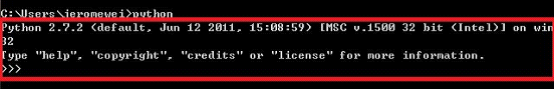
\includegraphics[width=10cm]{./runpython.png}
\caption{python运行}
\end{figure}
\end{document}
